%%%%%%%%%%%%%%%%%%%%%%%%%%%%%%%%%%%%%%%%%%%%%%%%%%%%%%%%%%%%%%%%%%%%%%%%%%%%%%%%%%%%%%%%%%%%%%%%%
%
% Document:     DM Support Prd.  product tree
%
%%%%%%%%%%%%%%%%%%%%%%%%%%%%%%%%%%%%%%%%%%%%%%%%%%%%%%%%%%%%%%%%%%%%%%%%%%%%%%
\documentclass{article}
\usepackage{times,layouts}
\usepackage{tikz,hyperref,amsmath}
\usetikzlibrary{positioning,arrows,shapes,decorations.shapes,shapes.arrows}
\usetikzlibrary{backgrounds,calc}
\usepackage[paperwidth=46.800000000000004cm,paperheight=3.62cm,
left=-2mm,top=3mm,bottom=0mm,right=0mm,
noheadfoot,marginparwidth=0pt,includemp=false,
textwidth=30cm,textheight=50mm]{geometry}
\newcommand\showpage{%
\setlayoutscale{0.5}\setlabelfont{\tiny}\printheadingsfalse\printparametersfalse
\currentpage\pagedesign}
\hypersetup{pdftitle={DM products }, pdfsubject={Diagram illustrating the
                products in LSST DM }, pdfauthor={Autogenerated from MD}}
\tikzstyle{tbox}=[rectangle,text centered, text width=30mm]
\tikzstyle{wbbox}=[rectangle, rounded corners=3pt, draw=black, top color=blue!50!white,
                    bottom color=white, very thick, minimum height=12mm, inner sep=2pt,
                    text centered, text width=30mm]
\tikzstyle{pbox}=[rectangle, rounded corners=3pt, draw=black, top
 color=yellow!50!white, bottom color=white, very thick,
 minimum height=35pt, inner sep=2pt, text centered, text width=35mm]
\tikzstyle{pline}=[-, thick]
\begin{document}
\begin{tikzpicture}[node distance=0mm]


\node (BCI) [pbox, 
] {\textbf{Build and CI
} };
\node (CAM) [pbox, 
right=1.5cm of BCI] {\textbf{Cont. Application Mng
} };
\node (DDCPUB) [pbox, 
right=1.5cm of CAM] {\textbf{DM Doc Publication
} };
\node (DDVSRV) [pbox, 
right=1.5cm of DDCPUB] {\textbf{DM Dev Services
} };
\node (DEPLOY) [pbox, 
right=1.5cm of DDVSRV] {\textbf{SW Deployment
} };
\node (DMDCOM) [pbox, 
right=1.5cm of DEPLOY] {\textbf{Devlop. Comm
} };
\node (PKGDST) [pbox, 
right=1.5cm of DMDCOM] {\textbf{Packagin Distrib
} };
\node (SWVER) [pbox, 
right=1.5cm of PKGDST] {\textbf{SW Version Control
} };
\node (DMDSRV) [wbbox, above=15mm of DEPLOY]{\textbf{Support Services
}};
 \draw[pline]   (BCI.north) -- ++(0.0,0.5) -| (DMDSRV.south) ; 
 \draw[pline]   (CAM.north) -- ++(0.0,0.5) -| (DMDSRV.south) ; 
 \draw[pline]   (DDCPUB.north) -- ++(0.0,0.5) -| (DMDSRV.south) ; 
 \draw[pline]   (DDVSRV.north) -- ++(0.0,0.5) -| (DMDSRV.south) ; 
 \draw[pline]   (DEPLOY.north) -- ++(0.0,0.5) -| (DMDSRV.south) ; 
 \draw[pline]   (DMDCOM.north) -- ++(0.0,0.5) -| (DMDSRV.south) ; 
 \draw[pline]   (PKGDST.north) -- ++(0.0,0.5) -| (DMDSRV.south) ; 
 \draw[pline]   (SWVER.north) -- ++(0.0,0.5) -| (DMDSRV.south) ; 

\end{tikzpicture}
\end{document}
